%
% File main.tex
%
% Contact: car@ir.hit.edu.cn, gdzhou@suda.edu.cn
%%e.agirre@ehu.es or Sergi.Balari@uab.es
%% and that of ACL 08 by Joakim Nivre and Noah Smith

\documentclass[11pt]{article}
\usepackage{acl2015}
\usepackage{times}
\usepackage{url}
\usepackage{latexsym}
\usepackage{graphicx}
\usepackage{listings}

%\setlength\titlebox{5cm}

% You can expand the title box if you need extra space
% to show all the authors. Please do not make the title box
% smaller than 5cm (the original size); we will check this
% in the camera-ready version and ask you to change it back.


\title{Spoiler detection and extraction\\2nd Project Report for NLP Course, Winter 2022}

\author{M. Kierznowski, Ł. Pancer, P. Wesołowski \\
  Warsaw University of Technology \\
%   {\tt email@domain} \\
  \And
    supervisor: Anna Wróblewska \\
  Warsaw University of Technology \\
    {\tt anna.wroblewska1@pw.edu.pl}
    }

\date{}

\begin{document}
\maketitle
\begin{abstract}
This document presents the results of the second project for the Natural Language Processing course. The project addresses the spoiler detection task but in a non-standard way. Current research in this field mainly relates to review classification. Our approach focuses on phrase extraction. Namely, for a given review, we want to point out specific words that constitute spoilers. Alternatively, the task may be expressed as a token classification task, i.e., for every word in the review, the goal is to mark it as a spoiler or non-spoiler. Due to the definition and uniqueness of the problem, only one spoiler dataset offers sufficiently precise annotations. Moreover, no reference scores are available. We prepare deep learning models and verify their performance using the properly preprocessed dataset. Our experiments rely on LSTM and BERT-based models. We compare the impact of the use of attention and case-sensitive models. Finally, we provide ideas for further experiments.
\end{abstract}

\section{Introduction}

In everyday life, information that reveals the important aspects, events, and twists of a plot of, e.g., a book, a movie, or a videogame is referred to as a spoiler. Spoilers are usually undesired, and getting to know one of them may contribute to a decrease in enjoyment \cite{abbott2020can} or a lack of further interest in reading or seeing a particular position \cite{li2022exploring}. However, they can often become known by chance, for example, due to being a part of some review. Therefore, automatic spoiler detection has become one of the crucial tasks in the NLP field \cite{guo2010finding}.

Several methods on this issue have been proposed. However, the authors often focus on their text classification performance. Let us note that in the previous project, we developed models for the entire review classification. Then, we employed interpretability techniques and verified the model's rationale behind spoiler classification on the word level. In other words, we examined which words were the primary reason for classifying the entire text as a spoiler. Motivated by such research done in the previous project, we decided to go a little deeper into this problem. Instead of teaching our models to classify entire reviews and then extracting important phrases, we may teach the model directly to extract important phrases. The task may be interpreted as a word classification task or token classification task.



% Transfer learning has become popular in recent years due to possible better performance, shorter training time, hence lower electricity usage, or use of other, more readily available data \cite{torrey2010transfer,weiss2016survey}. However, proper fine-tuning on the task-related dataset may be important for further improvement in the model's robustness and accuracy. Similarly to our predecessors, we are going to utilize powerful pre-trained models. However, we would like additionally to make use of the IMDB reviews dataset \cite{enam_biswas_2021}. Although the smaller version is frequently used in the NLP tasks, its much larger variant, which we employ, is rarely utilized. We believe that due to its size (and, therefore, probably its diversity), it may be a good source of additional knowledge for our models.

Our project is driven mainly by the following questions: 
\begin{enumerate}
    \item Can we build a satisfactory model for spoiler phrase extraction? The question is motivated by the fact that such a model, provided that it offers sufficient performance, may be effectively incorporated into the business. Corresponding use cases could be found in various types of sites that allow the publication of reviews, comments, etc., on cultural works. We think that more precise tagging can be a better alternative than tagging and hiding the whole review from the reader. In our research, we want to provide some baseline models whose results can be, hopefully improved in the future.
    \item What is the impact of different language model properties on classification metrics? In particular, we compare attention and non-attention models. Furthermore, we examine the results of using both case-sensitive and case-insensitive models. One can expect that proper nouns, spelled with capital letters, might be one of the features helpful in identifying spoilers.
\end{enumerate}

The remainder of this work is organized as follows. Section \ref{related-work} provides a brief literature review. Section \ref{datasets} introduces the dataset utilized. Our approach is described in section \ref{approach}. Section \ref{experiments} presents the experiments conducted along with their results. The results obtained are further discussed in section \ref{discussion}. Finally, the conclusions and future work are presented in section \ref{conclusions}.

\section{Related work} \label{related-work}
Spoiler detection tasks had been previously neglected \cite{wan2019fine}, and only in recent years it saw more rapid development. Early studies related to spoiler detection treated it as a traditional classification task, most commonly utilizing methods such as Support Vector Machines. The progress revolved around the process of building a larger dataset with more linguistic features available. The previous works in this field explored basic Bag-of-Words approaches: creating a blacklist of words for a given topic \cite{golbeck2012twitter}, introducing temporal filtering system \cite{nakamura2007temporal}, using topic models based on Latent Dirichlet Allocation \cite{guo2010finding}. Significant contributions to publicly available datasets include TV Tropes Movies \cite{boyd2013spoiler} and Goodreads dataset \cite{wan2019fine}. Chang \shortcite{chang2018deep} proposed an attention-based solution, and today similar approaches still remain state-of-the-art. More recently, a transfer learning approach was suggested, laying the stress on interpretability, and introducing alongside a new dataset - TV Tropes Books \cite{wroblewska2021spoiler}.

One of the key models widely used in the NLP discipline is BERT \cite{devlin2018bert}, which stands for Bidirectional Encoder Representations from Transformers. Since its introduction, it has received much appeal for outperforming other methods in various NLP tasks. DistilBERT \cite{sanh2019distilbert} is a slim implementation of BERT, containing about 60\% of BERTs parameters. The authors, as well as the empirical results, suggest a 60\% speedup in reference to BERT while retaining slightly worse yet comparable results. 

Our current project idea was inspired by a medium article \cite{medium_extract}, an overview of a solution to a Twitter sentiment extraction Kaggle competition \cite{kaggle_comp}. The competition brought up the subject of extracting the exact part of a sentence responsible for its sentiment. For example, in a tweet, "my boss is bullying me," the phrase "bullying me" is directly responsible for its negative sentiment, as the rest of the sentence is neutral and could be used in a sentence of any sentiment. A lot can be discovered from problems of similar nature. 

Zhang \shortcite{zhang2011extracting} proposed a method for selecting words that do not bear sentiment on their own but only given context. For example, words describing resources may be positive or negative, e.g., "The washer uses a lot of electricity" or "The washer uses little water." Yet another work \cite{rezaeinia2017improving} introduces an Improved Word Vectors (IWV) method, improving the accuracy of pretrained word embeddings. Jianqiang et al. in \shortcite{jianqiang2018deep} applied a word embeddings method to sentiment analysis of Twitter posts. It's an improvement over TF-IDF because it extracts features such as contextual semantic relationships and co-occurrence statistical characteristics between words. Their approach, based on deep convolutional neural networks, outperformed the baseline word n-gram models. In \cite{madasu2020efficient}, authors study the impact of a number of machine learning classifiers on the Term Frequency Inverse Document Frequency (TF-IDF) technique. Using feature selection combined techniques, they were able to outperform neural networks in sentiment analysis.




\section{Dataset} \label{datasets}
In our research, contrary to the previous project, we utilized only one dataset. This stems from the fact that only this one offers word-level annotations. The characteristics of this dataset are as follows:
\begin{itemize}
\item TV Tropes Books\footnote{available at \url{https://github.com/rzepinskip/tvtropes-books}} - 340k documents, 670k sentences, 110k spoiler sentences, 1:4 spoiler to non-spoiler reviews.
\end{itemize}

The dataset is already split into the training (80\%), validation (10\%), and testing (10\%) parts. A sample from the dataset is presented in listing~\ref{lst:sample-tvtropes-books}.
Further exploratory data analysis is provided in section \ref{eda}.

\begin{figure*}[h]
\begin{lstlisting}[basicstyle=\small,caption={Sample JSON object in the TV Tropes Books dataset. Each sentence contains a boolean flag that identifies spoiler sentences. In addition, annotated character indices provide specific spoiler boundaries - in the case depicted, the spoiler spans indexes from 0 to 89.},label={lst:sample-tvtropes-books}]
{
'page': 'https://tvtropes.org/...',
'trope': 'Kill the Cutie',
'has_spoiler': True,
'sentences': [[True, 'Walter, who was the ...', [[0, 89]]]]
}
\end{lstlisting}
\end{figure*}





\section{Approach} \label{approach}

In general, our methodology consists of the following points:
\begin{itemize}
\item Preprocess the dataset. The raw dataset contains spoiler annotations but it has to undergo transformation to be ready to be processed by models.
\item Create and verify the performance of LSTM-based models.
\item Create and verify the performance of state-of-the-art BERT-based models.
\end{itemize}

In line with our previous project, apart from employing LSTM architectures, we have focused on state-of-the-art solutions based on transformer architecture. Apart from exploring the standard BERT model, we decided to try smaller DistilBERT architecture. Due to our computational limits, we felt it would be better to go this way rather than larger models such as the ELECTRA. 

Finally, it's worth noting that BERT models come in two versions - case sensitive and case insensitive. Our intuition tells us that words starting with a capital letter can characterise spoilers to a certain extent. Accordingly, we are testing both options.

% \begin{table}[h]
%     \centering
%     \begin{tabular}{|c|c|}
%         Model & \#Parameters \\\hline
%         DistilBERT & 66M \\
%         BERT & 110M
%     \end{tabular}
%     \caption{Comparison of used BERT-based base architectures}
%     \label{tab:bert-comparison}
% \end{table}

We treat the phrase extraction as a token classification task. Every model has a fixed maximum number of input tokens. Furthermore, the models feature the same number of output neurons. Every neuron outputs a number in the $[0, 1]$ interval being a probability that a corresponding word is a spoiler. For clarity, the 1st neuron outputs the probability of being a spoiler for a 1st token, the 2nd neuron the probability for the 2nd token, etc. Due to the fixed maximum input token number, the dataset has to be properly preprocessed. We have to make sure that our input samples are not longer than the specified number of tokens. The algorithm, motivated by the exploratory data analysis presented later, is as follows. For every spoiler review, perform the following operations:
\begin{enumerate}
\item Concatenate sentences as long as they are within the maximum number of words.
\item Add concatenated sentences to the final dataset.
\item If some sentences from the review considered have not been included in the result, go back to 1. and start concatenating them.
\end{enumerate}
Of course, single sentences that are longer on their own than the maximum number of words allowed are not included in the resulting dataset. It is worth noting that this transformation must be combined with procedures typically performed by a tokenizer, such as splitting. It's due to the need to track the positions of spoiler words. Therefore, simultaneously with the concatenation operations, the target label vector is created. The length of the vector equals the number of words in the corresponding review fragment. Such a vector contains boolean flags indicating spoiler words. Example data and corresponding target vector are presented in listing \ref{lst:sample-final-data}.

\begin{figure*}[t]
\begin{lstlisting}[basicstyle=\small,caption={Sample element of the dataset adjusted to our needs. The maximum number of tokens in this case was 64. Note that the text has already undergone preprocessing, e.g., punctuation removal. The target vector is a boolean vector indicating spoiler words. In this case, \textit{and can't bear him children} was annotated as a spoiler phrase.},label={lst:sample-final-data}]
("celia is this to johnny because he's from a rich well to do family while she's
white trash from sugar ditch and doesn't know how to cook clean and can't bear him
children",
 [False, False, ..., False, True, True, True, True, True])
\end{lstlisting}
\end{figure*}


One important remark needs to be elaborated on. As stated, we decided to use LSTM and BERT-based models. While our custom tokenization procedure, which allows to annotate each token as a spoiler or non-spoiler, may be used to tokenize the input for LSTM layer, a tokenization for BERT models differs slightly. In particular, BERT tokens include subword tokens (the common notation is to precede them with double hash symbol). This type of token results from the greedy extraction of known fragments from unknown words. This, in turn, has some impact on our models. We have to adjust our labeled split into words datasets so that they correspond to the BERT tokens. In particular, we have used BERT tokenizer on already split and labeled tokens. This sometimes led to further split of tokens, e.g., \textit{characteristically} $\to$ \textit{characteristic} and \textit{\#\#ally}. Let us stress that in this process, we handle our token labels correctly. In the example provided, if the \textit{characteristically} was annotated as a spoiler, then both two resultant tokens will be labelled as spoilers. Similarly for non-spoilers.

The above comment indicates that the datasets on which the models are evaluated on are not entirely the same for LSTM and BERT models. The differences are not significant and are due to the presence of subword tokens.

Another important remark in relation with regard to our models relates to correct approach to padding. Note that our models, by definition, have a fixed number of output neurons. The relevant input text may contain fewer tokens. Still, the probabilities of being a spoiler are calculated also for additional padding tokens. Our initial experiments with an ordinary loss and metrics did not indicate any errors. However, in this case the input was limited to maximum 64 tokens. When we increased the number of possible tokens processed by the model to 512, our model optimization no longer makes sense. This was due to large number of padding tokens considered in calculations. Hence, we included masking in our models. The mask ensures that the loss, metrics, and other necessary parameters are calculated only for the relevant tokens. This applies in particular to the LSTM model, since the BERT architectures already contain masking and in this case it is sufficient to provide appropriate labelling. 


\subsection*{LSTM}
As already mentioned, in this approach, we use LSTM models with an embedding layer. It is responsible for transforming the tokenized input into predefined vectors. For initial vectors, we have selected the GloVe vectors with a length of one hundred. Let us mention that this layer was not trainable during the training process. This architecture was the basic approach to the problem. We wanted to improve it by adding some more advanced mechanisms to already working solutions. To achieve that, we incorporated the attention layer in the architecture by adding it at the near end of the model. This feature adjusts importance to specific parts of the input data while ignoring the rest to mimic the cognitive attention process. It may potentially lead to better results during work.

Overall, the vanilla LSTM (without attention) was composed of an embedding layer followed by two bidirectional LSTM layers and a final dense layer. Recurrent layers returned sequences, not a single vector. In the case of attention LSTM, it featured one more bidirectional LSTM layer followed by an attention layer, dropout with 0.1 rate (without it, we observed overfitting), and a final dense layer.


\subsection*{Transformers}

The second group of models is state-of-the-art transformers. For this task, we have selected standard BERT architecture and a smaller DistilBERT variant - both from the hugging face python library. At the end of those two architectures, we add a dense layer to obtain the needed output size. This approach makes it possible to utilize transformer models.

% On top of the base architecture, we use a single fully-connected linear layer preceded by a dropout. Pooled BERT outputs serve as input for the dropout layer and final classification head. Because of the potential time advantages of DistilBERT, in addition to accuracy scores, we also compare the running times of the two models. We verify whether it agrees with expectations and what the impact is on performance results.




\section{Experiments and results} \label{experiments}
\subsection{Exploratory data analysis} \label{eda}

The dataset contains serialized JSON objects. Recall that our final model has a fixed input tokens count and the same size output vector. Therefore, our exploratory data analysis was focused on choosing the right strategy to transform this dataset into a form that meets our expectations. The following exploratory data analysis is based on the training part of the dataset.

First, we decided to verify how many spoilers are annotated in a single sentence. Figure \ref{fig:spoilers-per-sentence} shows the corresponding histogram.

\begin{figure}
    \centering
    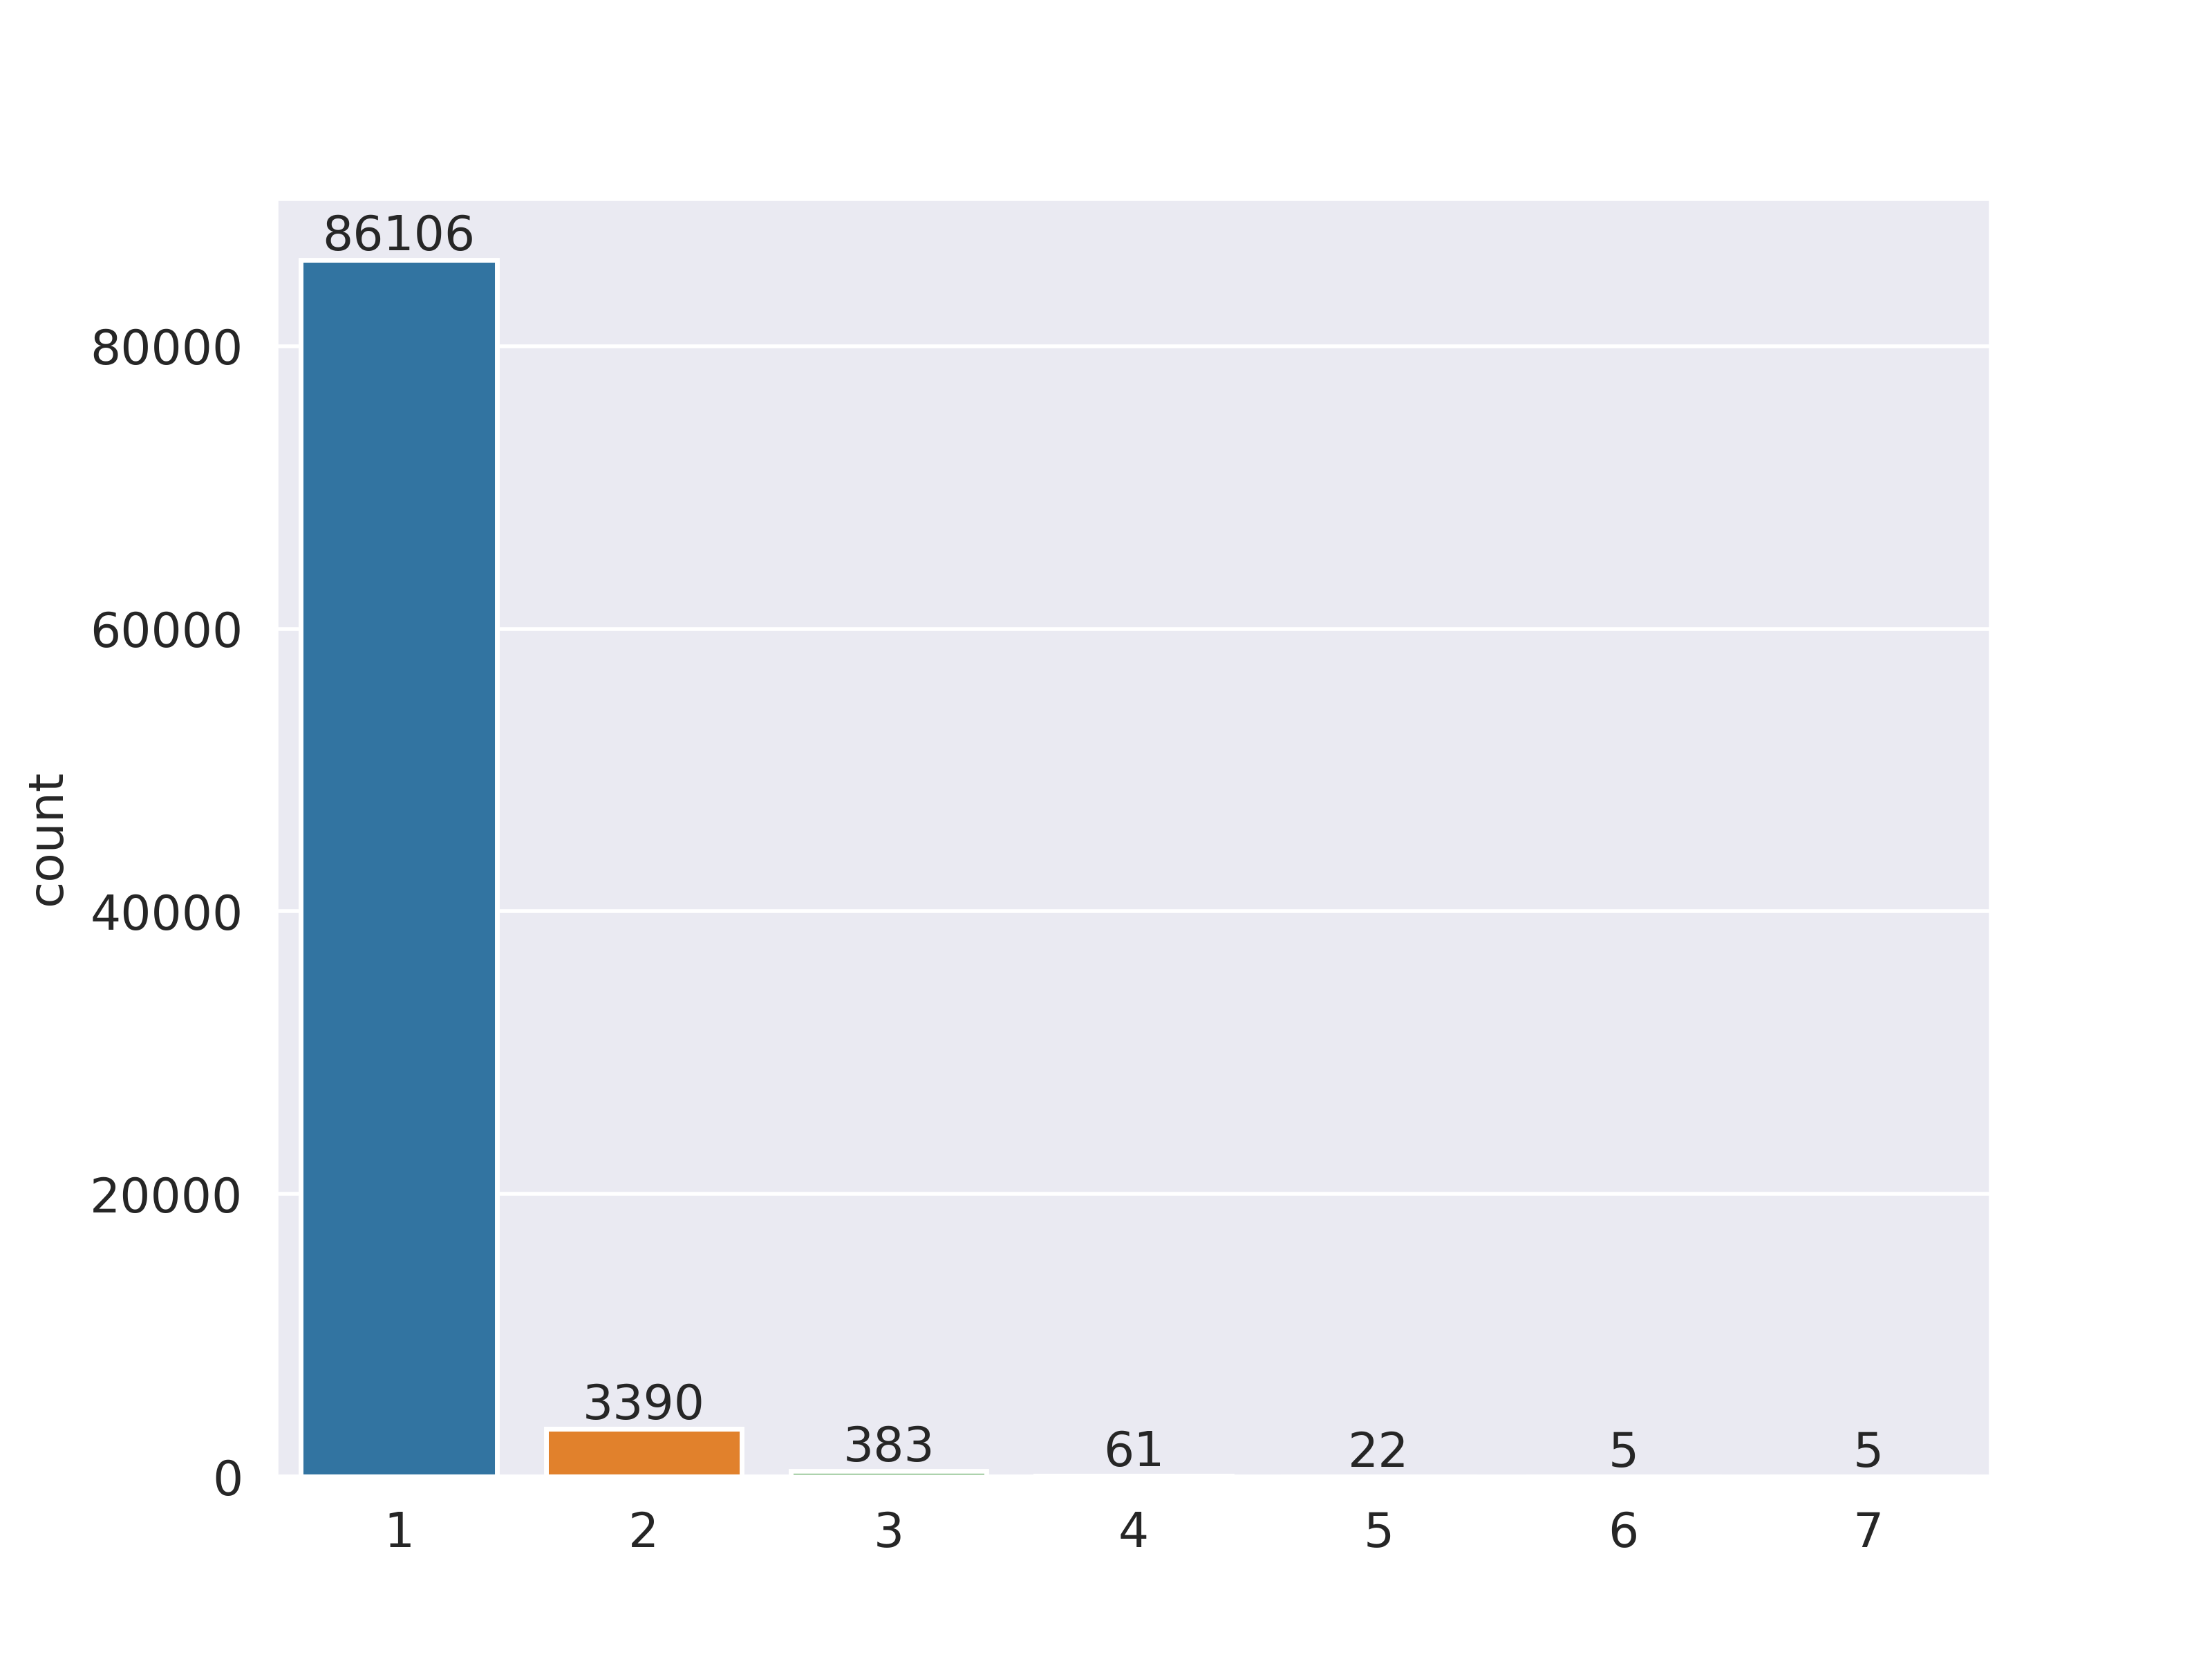
\includegraphics[width=\columnwidth]{img/eda/spoilers_per_sentence.png}
    \caption{Histogram presenting the distribution of spoiler counts within sentences. Note that only sentences with at least one spoiler are included. Sentences containing only one spoiler dominate.} 
    \label{fig:spoilers-per-sentence}
\end{figure}

Then, due to the expected fixed input word count, we focused on the histograms of the word count. Figure \ref{fig:words_count_per_spoiler_review} shows the histogram of word counts in the whole spoiler reviews. Another perspective is provided in figure \ref{fig:word_count_per_sentence_in_spoiler_review} depicting the histogram of word counts in sentences (only the sentences in spoiler reviews are considered). 

\begin{figure}
    \centering
    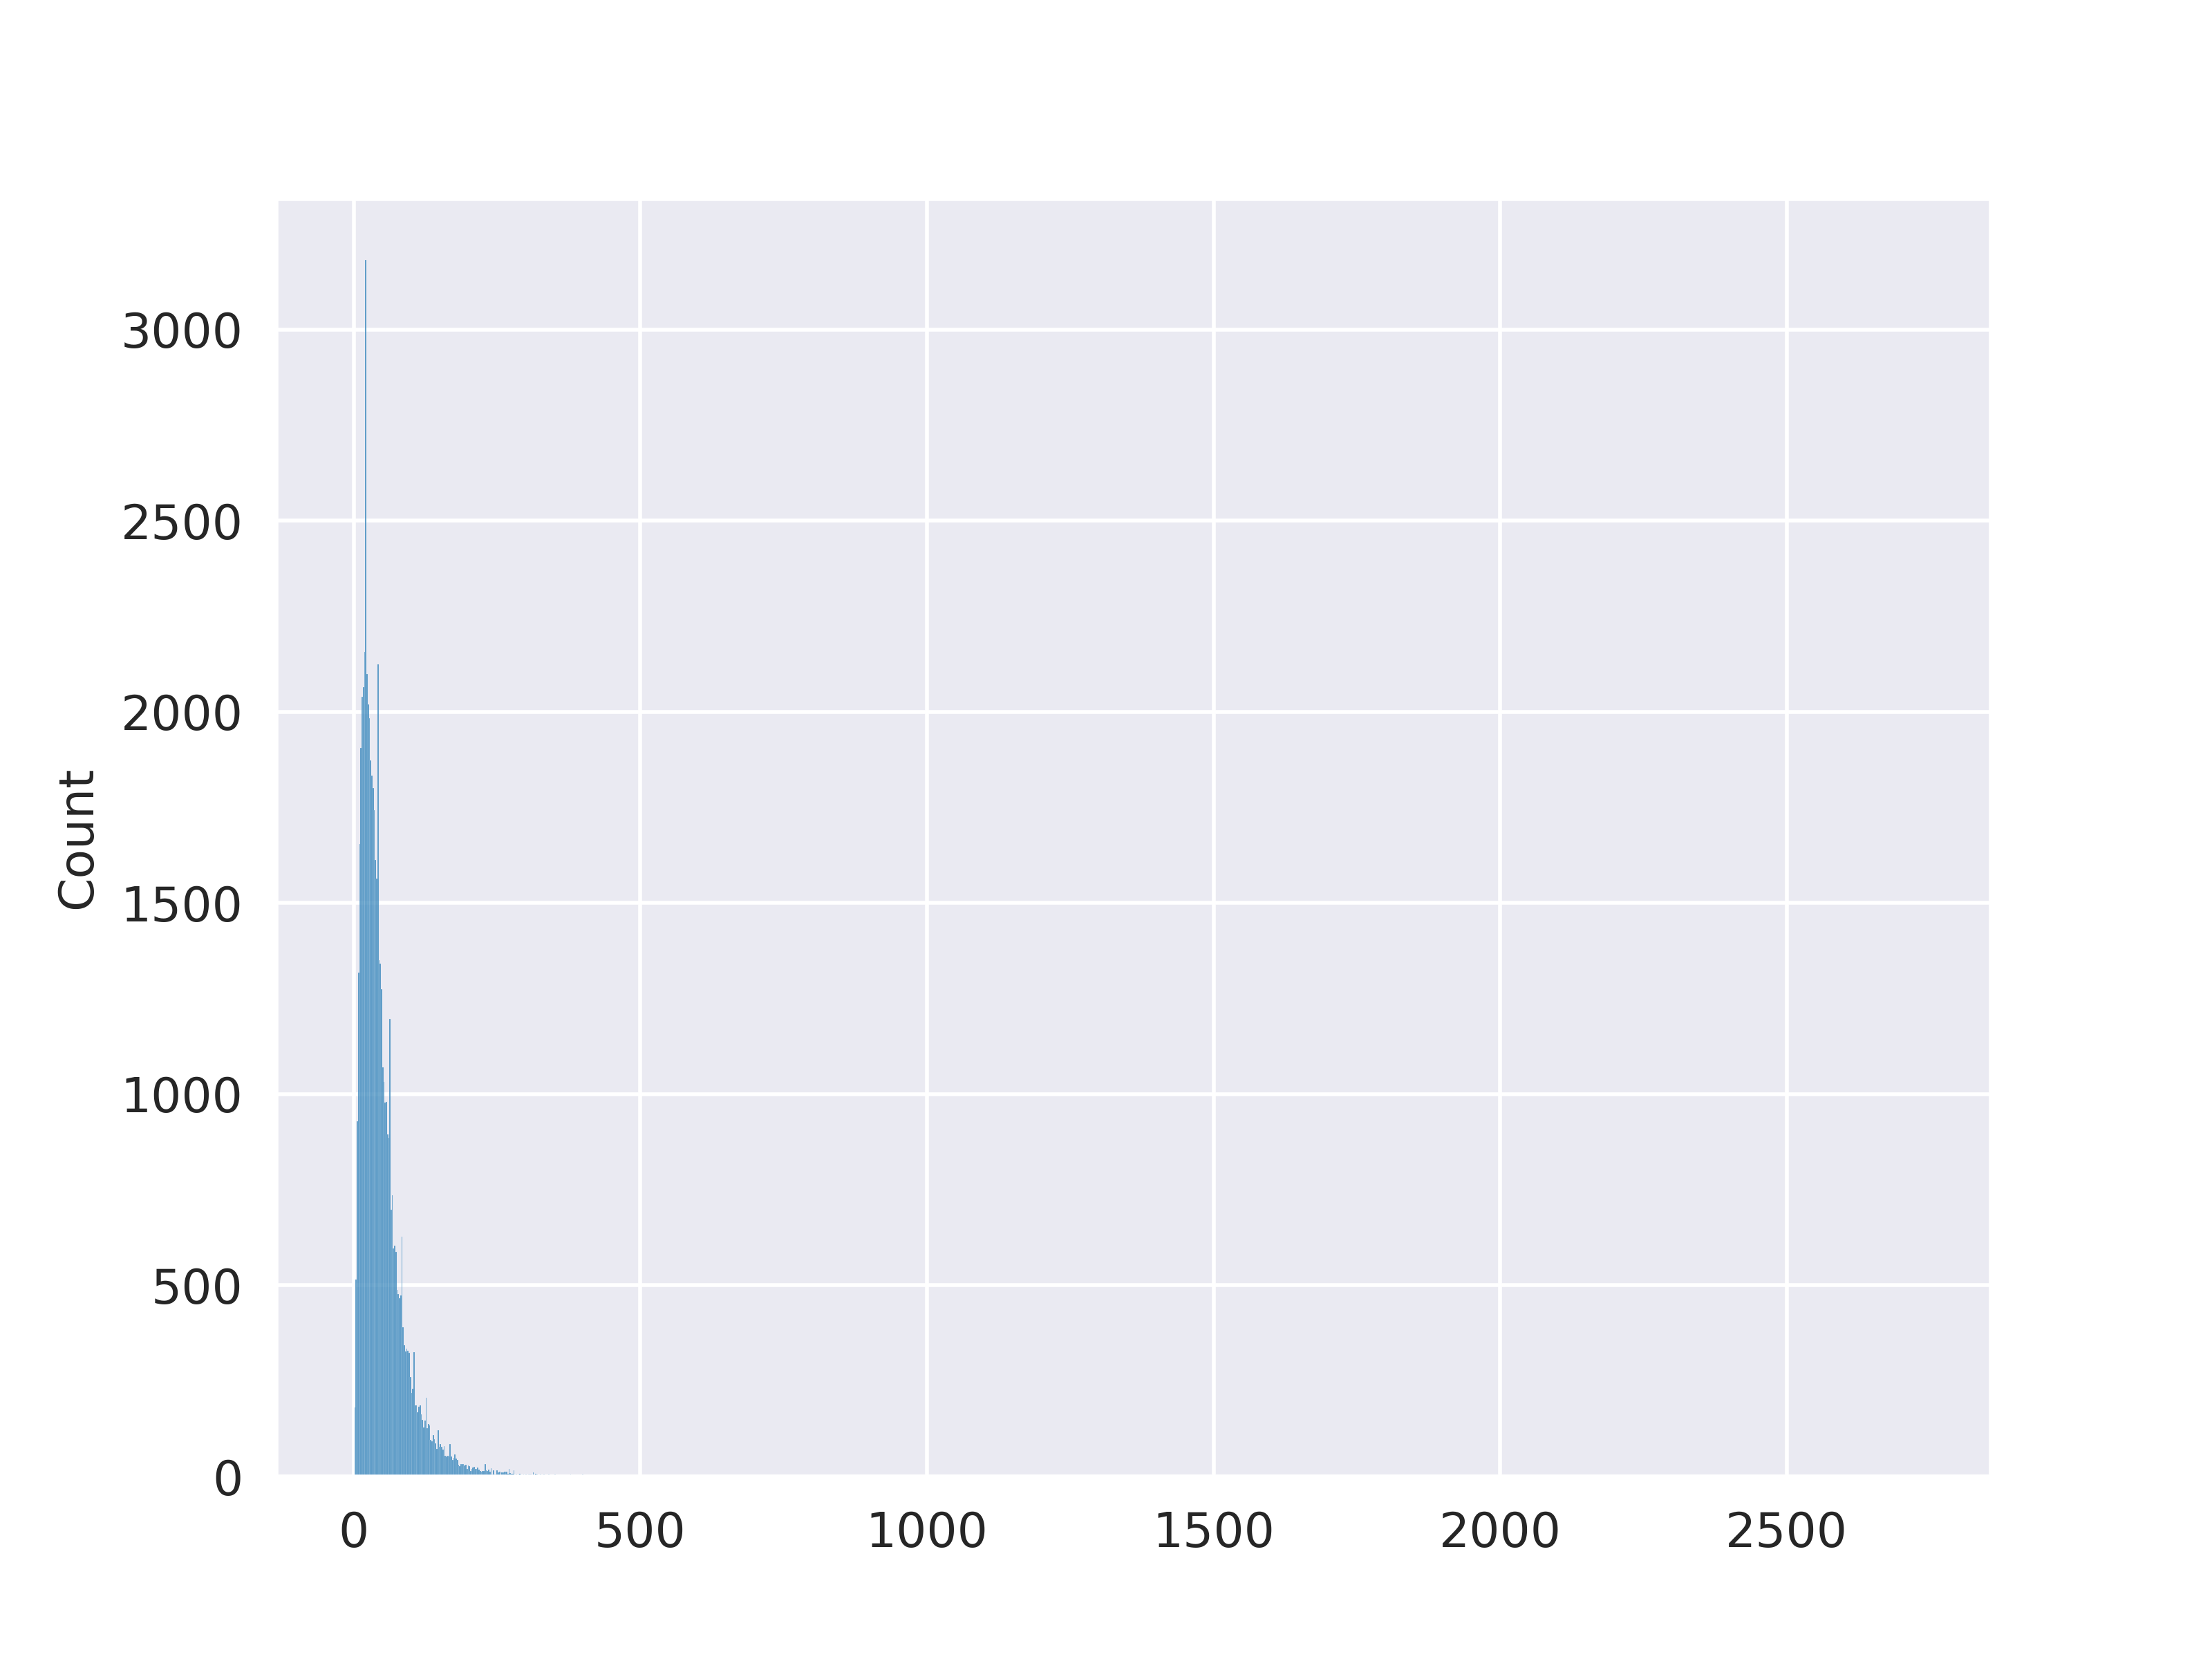
\includegraphics[width=\columnwidth]{img/eda/word_count_per_spoiler_review.png}
    \caption{Histogram presenting the distribution of word counts in whole spoiler reviews.} 
    \label{fig:words_count_per_spoiler_review}
\end{figure}

\begin{figure}
    \centering
    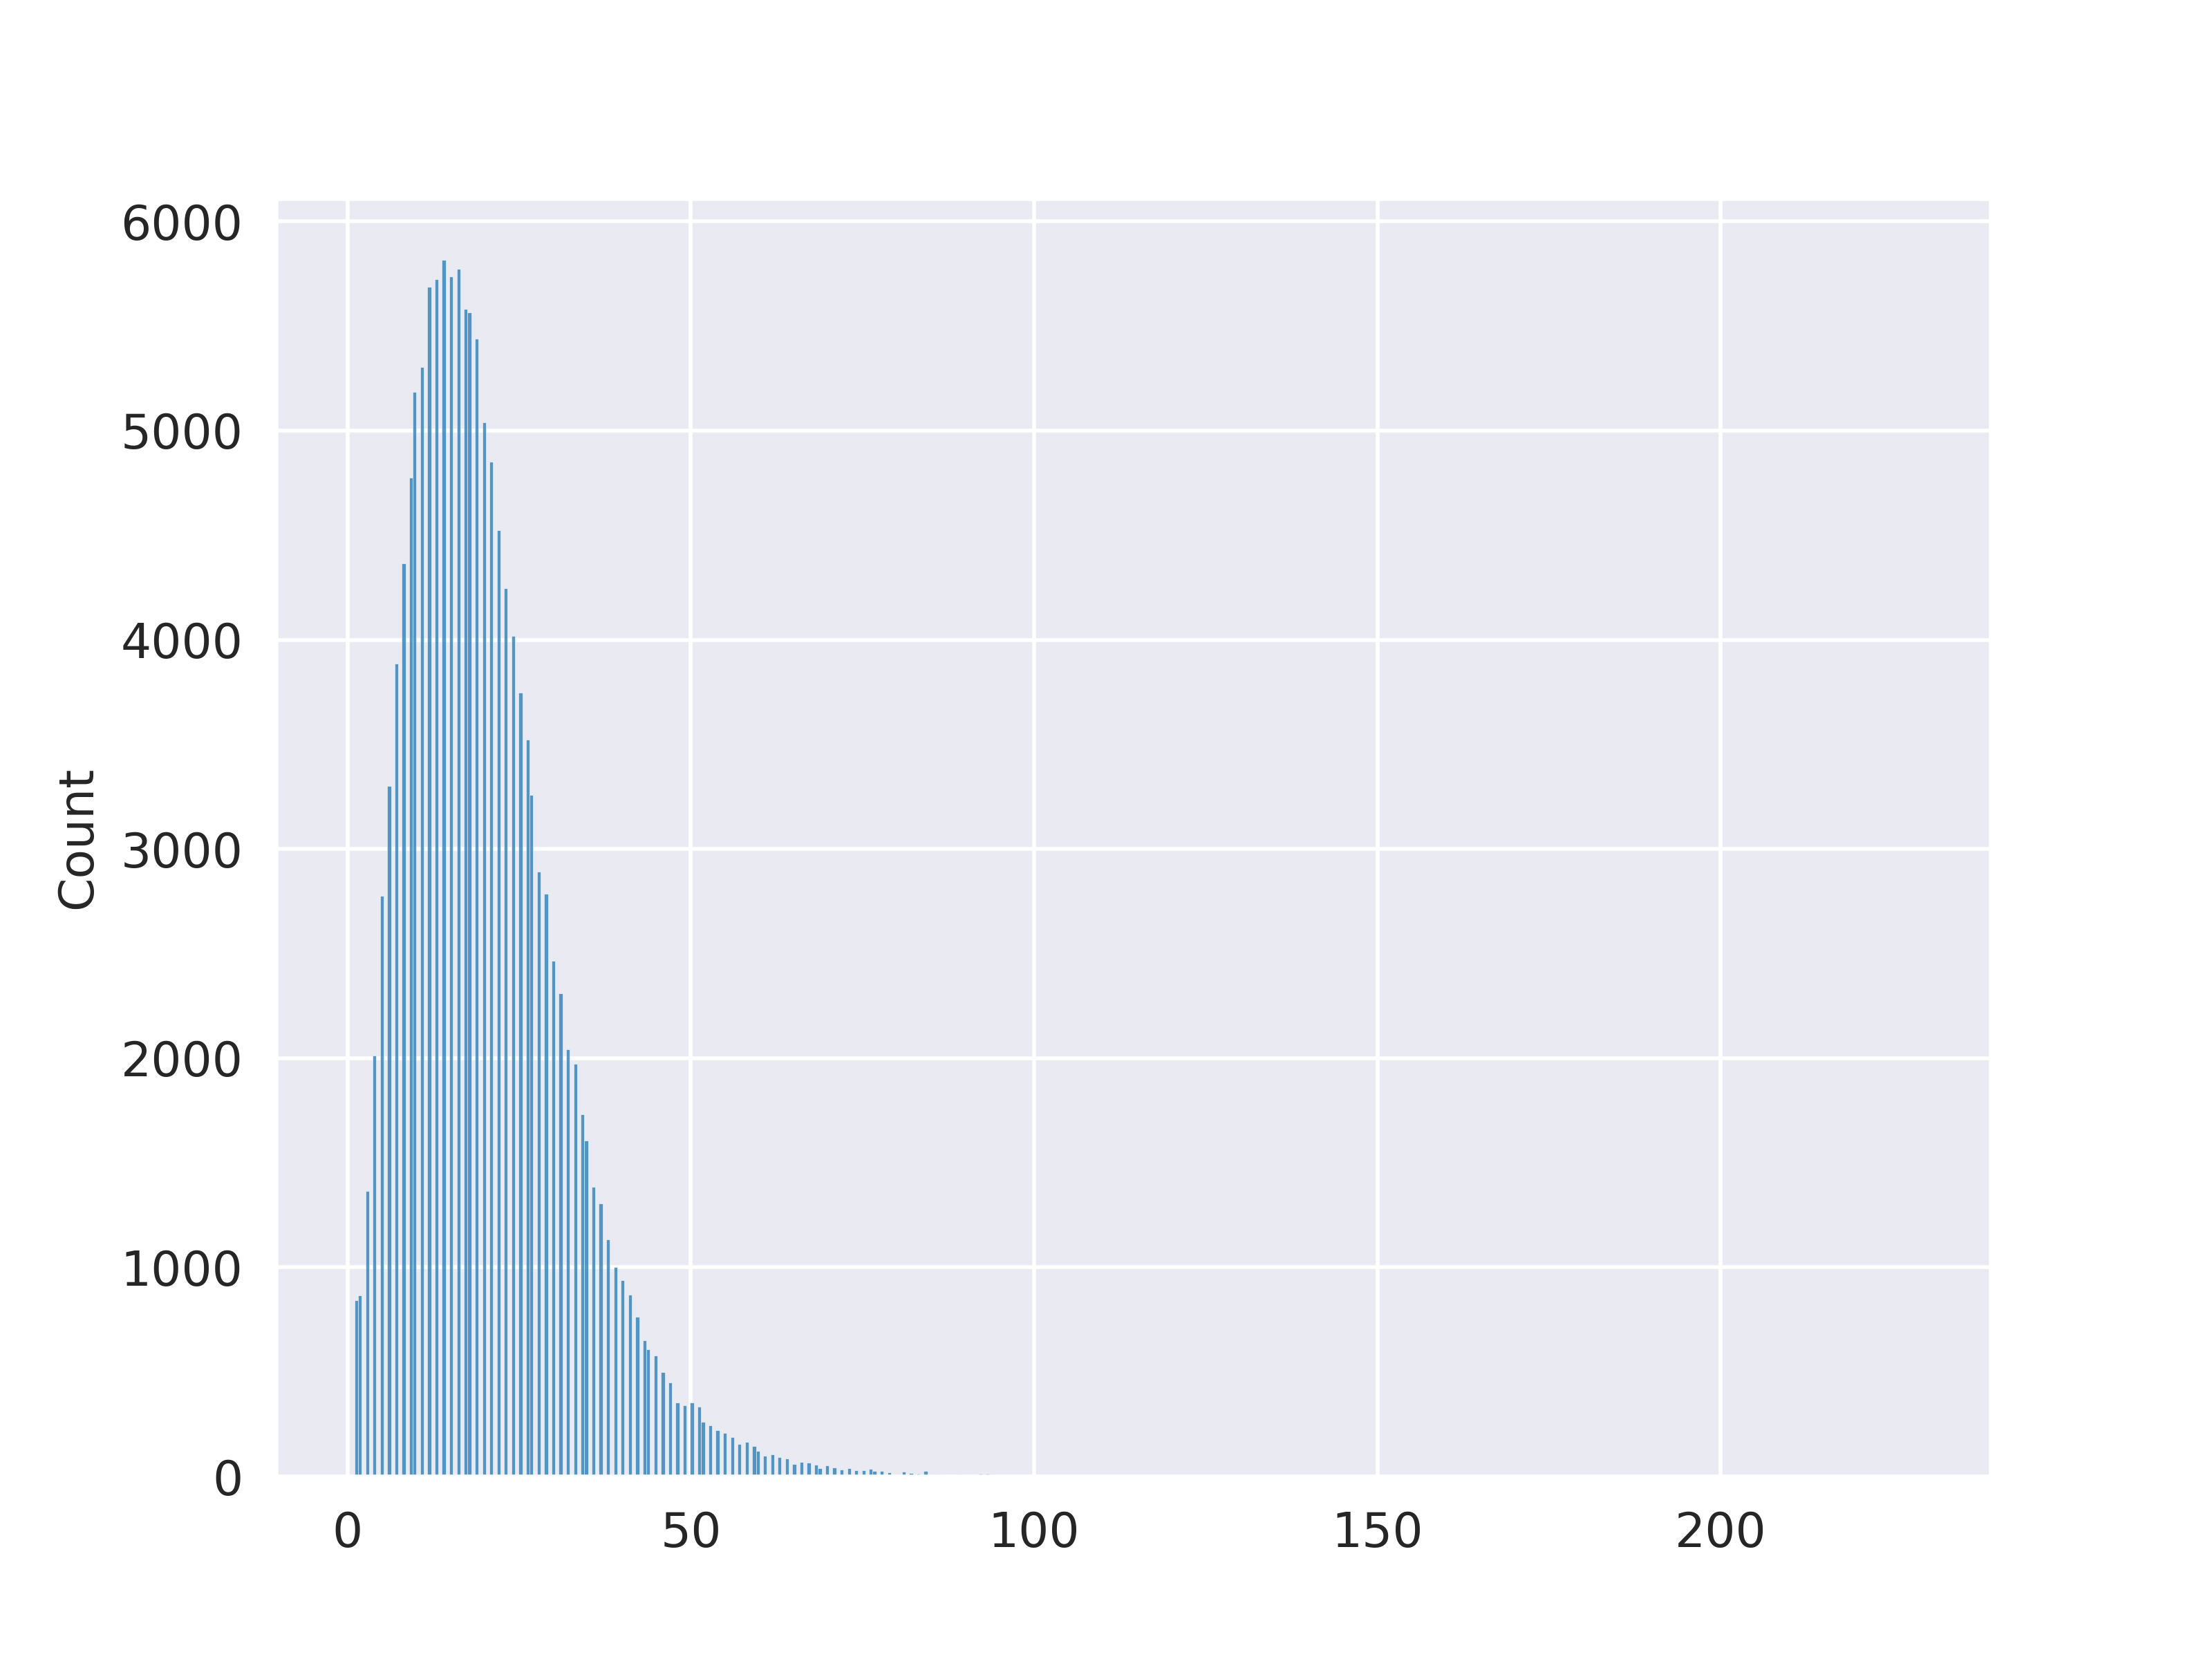
\includegraphics[width=\columnwidth]{img/eda/word_count_per_sencence_in_spoiler_review.png}
    \caption{Histogram presenting the distribution of word counts in sentences. The sentences come from spoiler reviews.} 
    \label{fig:word_count_per_sentence_in_spoiler_review}
\end{figure}

As we were looking for an idea of how to transform the collection appropriately to get review fragments with a certain maximum word count, we decided to check where in the sentences the spoilers end up. The result is shown in figure~\ref{fig:on_which_word_in_sentence_spoiler_ends}.
\begin{figure}
    \centering
    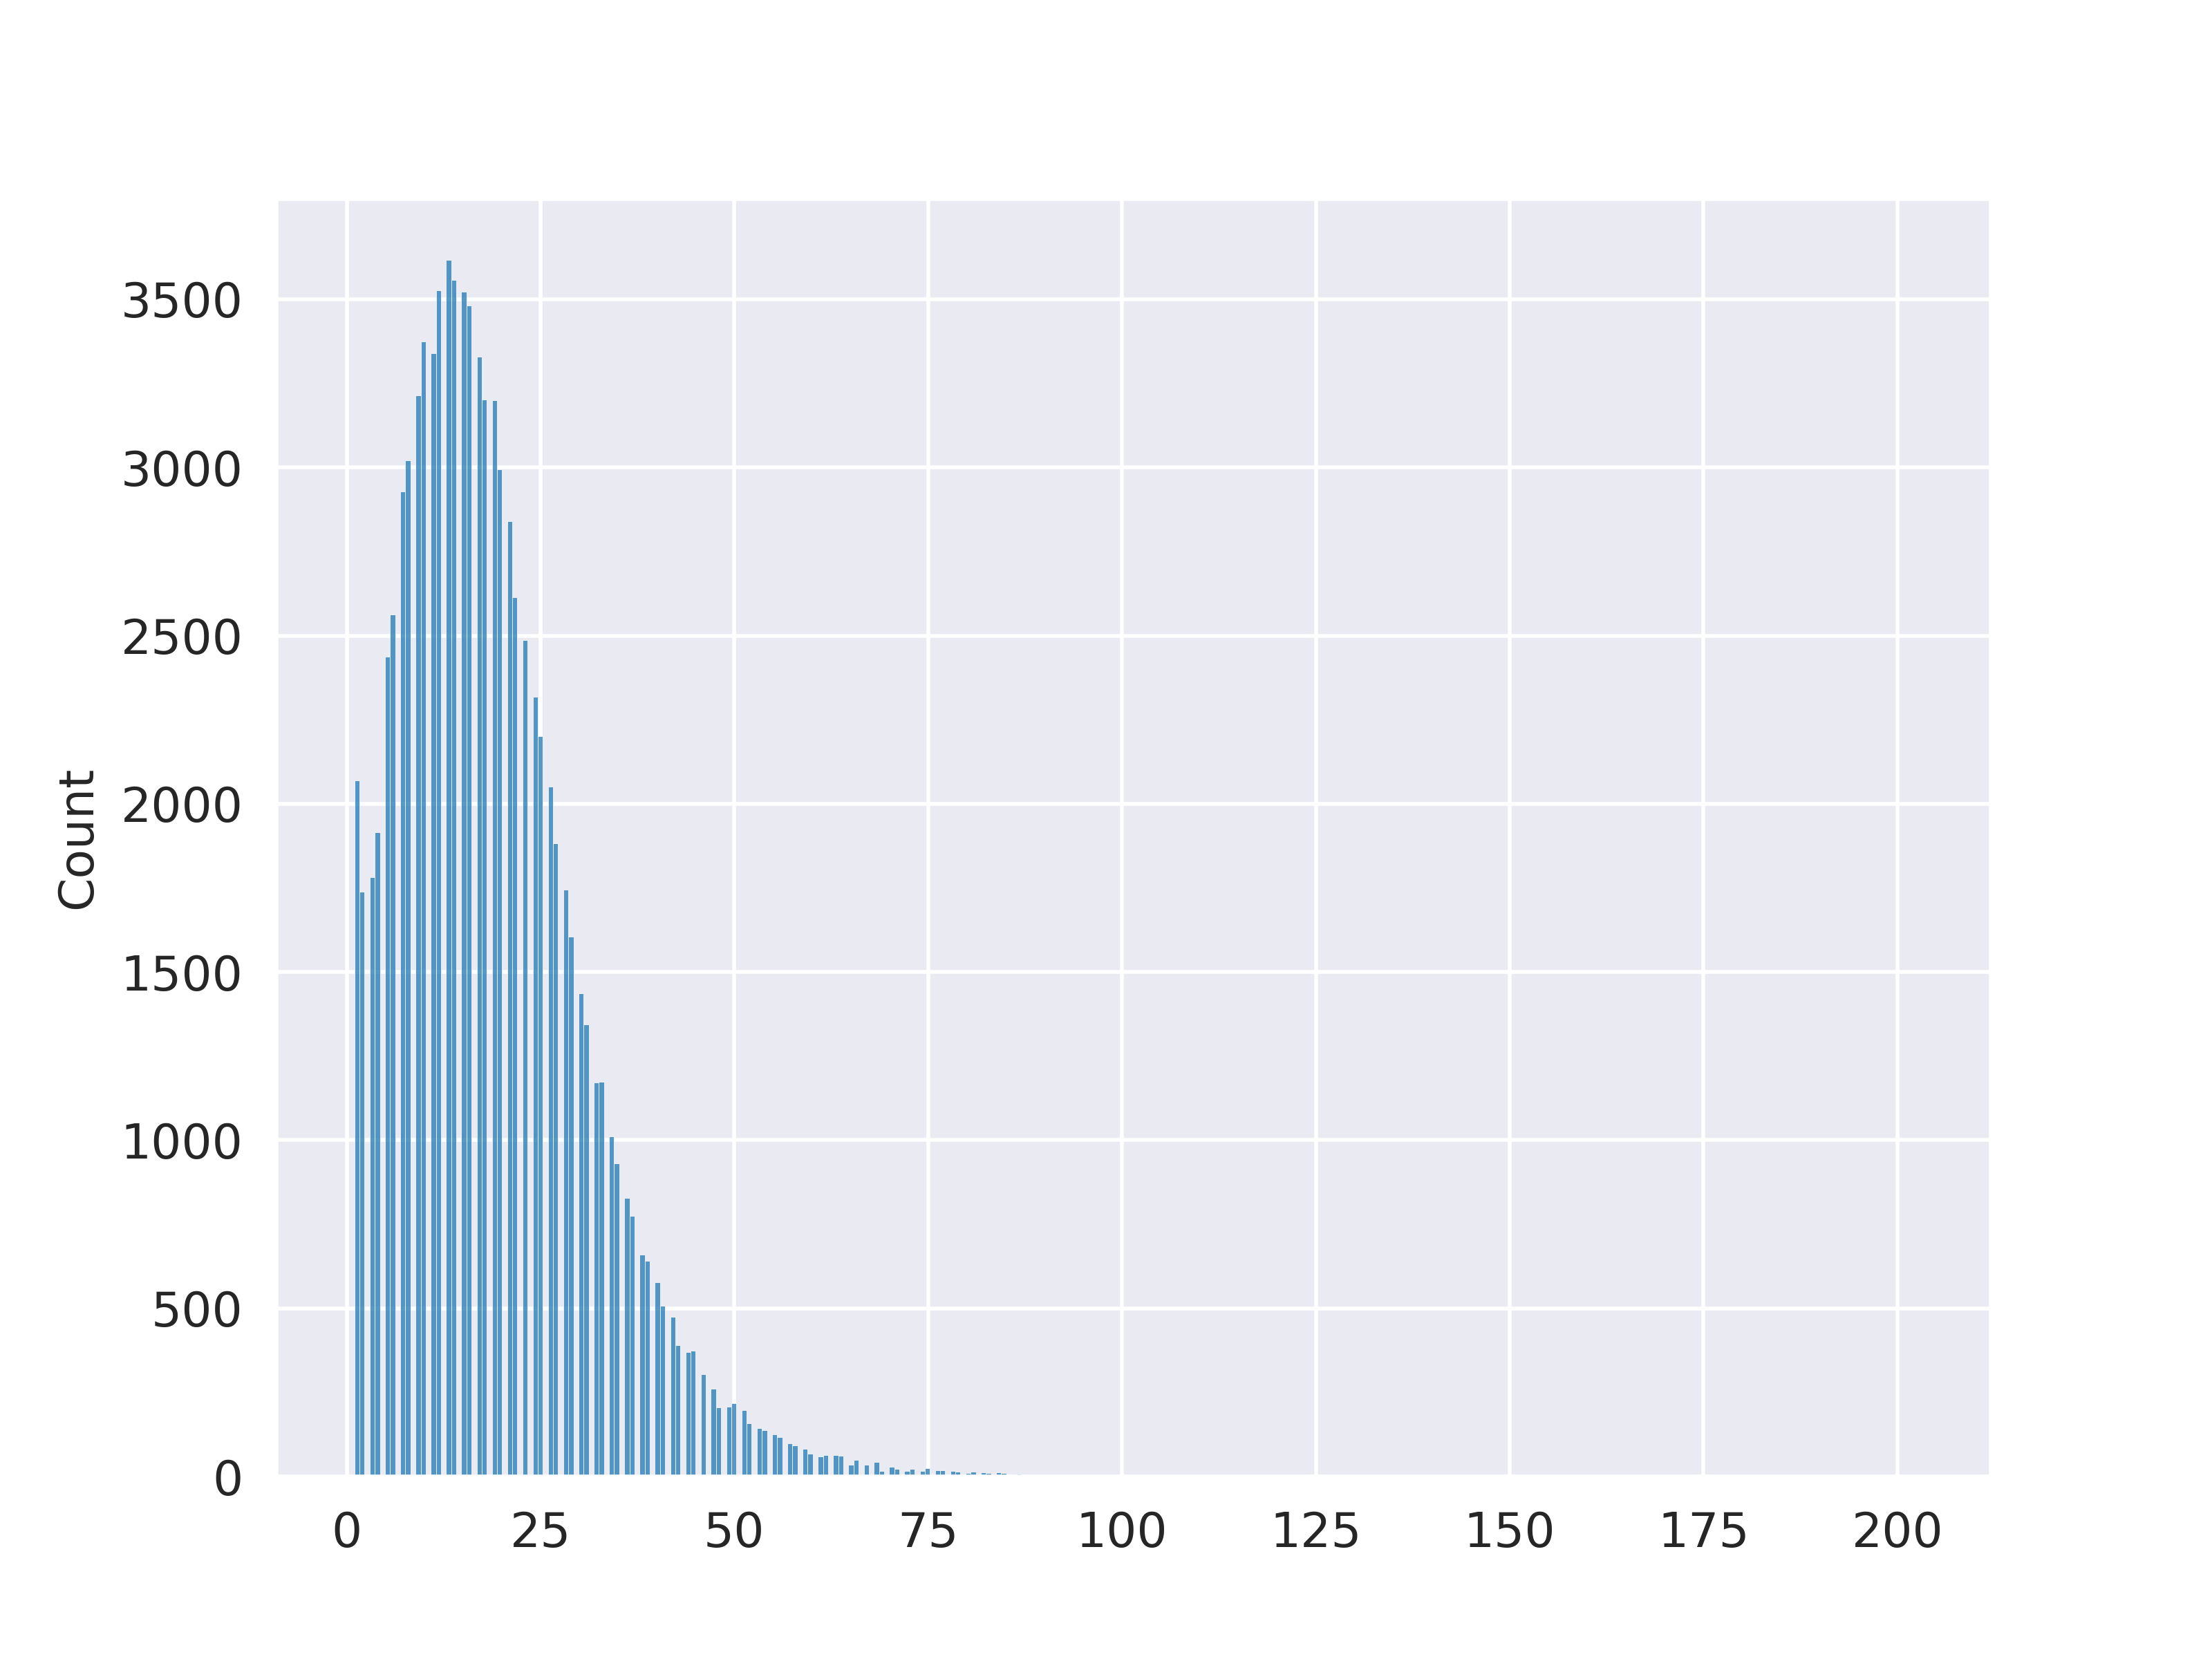
\includegraphics[width=\columnwidth]{img/eda/on_which_word_in_sentence_spoiler_ends.png}
    \caption{Histogram presenting the distribution of the last spoiler word inside a spoiler sentence.} 
    \label{fig:on_which_word_in_sentence_spoiler_ends}
\end{figure}

The similarity of figures \ref{fig:word_count_per_sentence_in_spoiler_review} and \ref{fig:on_which_word_in_sentence_spoiler_ends} seemed suspicious to us. Therefore, we decided to verify what fractions of spoiler sentences are actually annotated as spoilers. For every spoiler sentence, the number of words annotated as spoilers is divided by the number of words in the sentence. The histogram shown in figure \ref{fig:how_much_of_spoiler_is_in_spoiler_sentence} shows the distribution of these fractions.

\begin{figure}
    \centering
    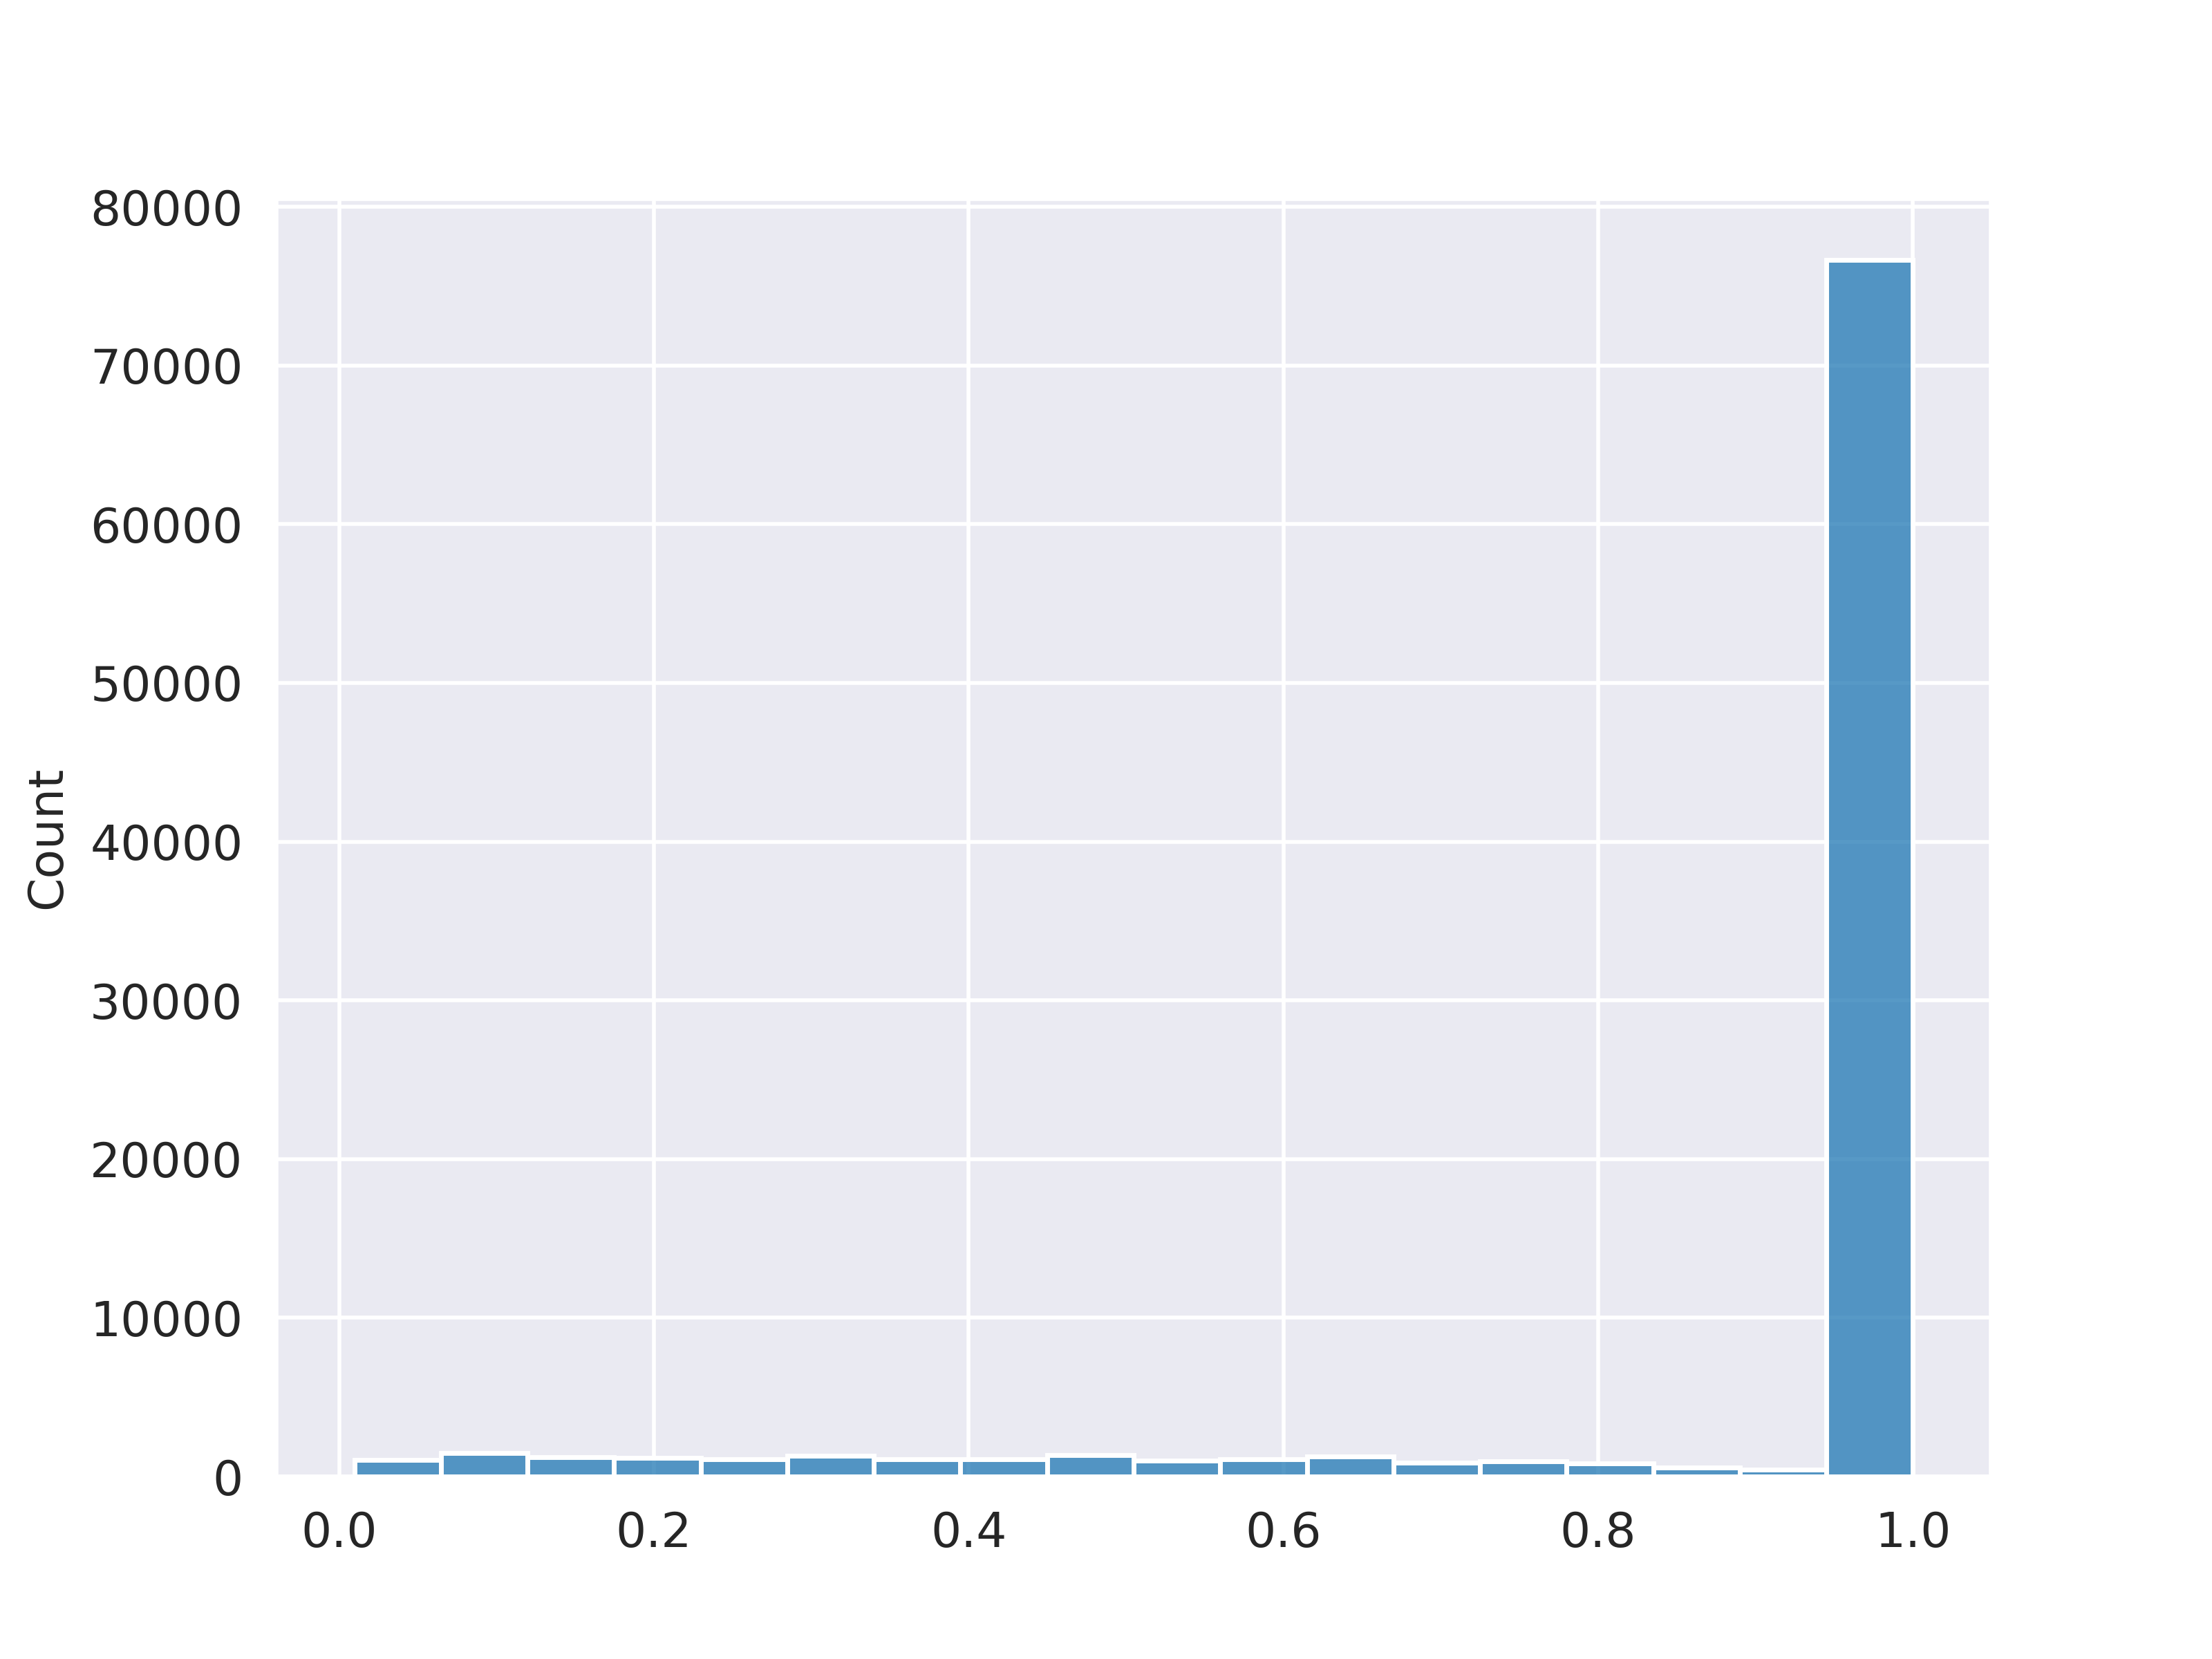
\includegraphics[width=\columnwidth]{img/eda/how_much_of_spoiler_is_in_spoiler_sentence.png}
    \caption{Histogram presenting the distribution of the fraction of spoiler words in spoiler sentences.} 
    \label{fig:how_much_of_spoiler_is_in_spoiler_sentence}
\end{figure}

The plot presented in figure \ref{fig:how_much_of_spoiler_is_in_spoiler_sentence} may be surprising. It turns out that in the vast majority, entire sentences are spoilers. We do not know whether this is due to fairly general tagging by portal users who have tagged whole sentences or whether whole sentences are actually spoilers.


\subsection{Training the models}
During our experiments, we utilized the TensorFlow library \cite{abadi2016tensorflow} and the Transformers library \cite{wolf2020transformers}, which provided the BERT models. Additionally, we used pre-trained weights for BERT-based models, but they were not frozen during training.

When it comes to LSTM models, they were trained with the following parameters. The hidden dimension of LSTM layers in both cases (without and with attention) was set to 256. The minibatch size was set to 32. Adam optimizer with the default parameters - 0.001 initial learning rate was used. We also tested some other values but observed no significant difference. The models were trained for 5 epochs, and the models with the largest validation accuracy were chosen. The results of the final models calculated on the test set are presented in table \ref{tab:resultsLSTM}. In the case of evaluation metrics selected, a spoiler class is $1$, non-spoiler is $0$. All metrics are calculated per word. For example, an accuracy of 70\% means that 70\% of words are correctly identified as spoilers or non-spoilers. \textit{Jaccard non-spoilers} corresponds to the Jaccard similarity score calculated between two sets of $0$ labels. Simirarly for \textit{Jaccard spoilers}.

We also trained BERT-based models. Note that due to our computational limits, the training possibilities were highly limited. Because of using pretrained weights, the models were trained using the optimizer used in HuggingFace examples, namely an Adam optimizer with an initial learning rate 2e-5, linear decay, and weight decay rate equal to 0.01. The minibatch size was set to 32, and models were trained for 3 epochs. The models with the best validation accuracy were tested on the test set, and the results are shown in table \ref{tab:resultsBertDistilBert}.




\begin{table*}[t]
\centering
\begin{tabular}{llllllllll}
\cline{1-6}
\multicolumn{1}{|c|}{Model}                  & \multicolumn{1}{c|}{Accuracy} & \multicolumn{1}{c|}{Recall} & \multicolumn{1}{c|}{Precision} & \multicolumn{1}{c|}{Jaccard non-spoilers} & \multicolumn{1}{c|}{Jaccard spoilers} &  &  &  &  \\ \cline{1-6}
\multicolumn{1}{|c|}{LSTM vanilla}           & \multicolumn{1}{c|}{0.6976}   & \multicolumn{1}{c|}{0.7402} & \multicolumn{1}{c|}{0.6478}    & \multicolumn{1}{c|}{0.5432}               & \multicolumn{1}{c|}{0.5278}           &  &  &  &  \\ \cline{1-6}
\multicolumn{1}{|c|}{LSTM + Attention layer} & \multicolumn{1}{c|}{0.7048}   & \multicolumn{1}{c|}{0.6526} & \multicolumn{1}{c|}{0.6857}    & \multicolumn{1}{c|}{0.5794}               & \multicolumn{1}{c|}{0.5024}           &  &  &  &  \\ \cline{1-6} 
\end{tabular}
    \caption{Results on the test set for LSTM models}
    \label{tab:resultsLSTM}
\end{table*}

\begin{table*}[t]
    \centering
\begin{tabular}{llllllllll}
\cline{1-6}
\multicolumn{1}{|c|}{Model}              & \multicolumn{1}{c|}{Accuracy} & \multicolumn{1}{c|}{Recall} & \multicolumn{1}{c|}{Precision} & \multicolumn{1}{c|}{Jaccard non-spoilers} & \multicolumn{1}{c|}{Jaccard spoilers} &  &  &  &  \\ \cline{1-6}
\multicolumn{1}{|c|}{DistilBERT uncased} & \multicolumn{1}{c|}{0.7055}   & \multicolumn{1}{c|}{0.4938} & \multicolumn{1}{c|}{0.7911}    & \multicolumn{1}{c|}{0.6183}               & \multicolumn{1}{c|}{0.4369}           &  &  &  &  \\ \cline{1-6}
\multicolumn{1}{|c|}{DistilBERT cased}    & \multicolumn{1}{c|}{0.7232}   & \multicolumn{1}{c|}{0.5814} & \multicolumn{1}{c|}{0.7640}    & \multicolumn{1}{c|}{0.6214}               & \multicolumn{1}{c|}{0.4929}           &  &  &  &  \\ \cline{1-6}
\multicolumn{1}{|c|}{BERT uncased}       & \multicolumn{1}{c|}{0.7120}   & \multicolumn{1}{c|}{0.5024} & \multicolumn{1}{c|}{0.8009}    & \multicolumn{1}{c|}{0.6248}               & \multicolumn{1}{c|}{0.4466}           &  &  &  &  \\ \cline{1-6}
\multicolumn{1}{|c|}{BERT cased}         & \multicolumn{1}{c|}{0.7205}   & \multicolumn{1}{c|}{0.5374} & \multicolumn{1}{c|}{0.7915}    & \multicolumn{1}{c|}{0.6280}               & \multicolumn{1}{c|}{0.4708}           &  &  &  &  \\ \cline{1-6} 
\end{tabular}
    \caption{Results on the test set for BERT and DistilBERT}
    \label{tab:resultsBertDistilBert}
\end{table*}





\subsection{In life comparison}

In order to assess the model performance in a more human-oriented, we verified the predictions on a few test samples by manually checking forecasts. This is an additional way to judge the prediction performance. To add another data source, we query the ChatGPT model to indicate spoilers in examples. Table \ref{tab:examplePrediction1} shows the real spoilers and models predictions in a sentence: \emph{Mila is quite interested in human society though she still prefers dolphins this starts to change as she regresses and she starts thinking more negative thoughts about humans}. Note that ground truth indicates the real spoilers. 

\begin{table*}[h]
    \centering
\begin{tabular}{llllllllll}
\cline{1-2}
\multicolumn{1}{|c|}{Source}         & \multicolumn{1}{c|}{Selected words as a spoilers}                                                                                                                   &  &  &  &  &  &  &  &  \\ \cline{1-2}
\multicolumn{1}{|c|}{Ground Truth}   & \multicolumn{1}{c|}{\begin{tabular}[c]{@{}c@{}}this starts to change as she   regresses and \\ she starts thinking more negative thoughts about human\end{tabular}} &  &  &  &  &  &  &  &  \\ \cline{1-2}
\multicolumn{1}{|c|}{Attention LSTM} & \multicolumn{1}{c|}{\begin{tabular}[c]{@{}c@{}}she regresses and she starts   thinking \\ more negative thoughts about humans\end{tabular}}                         &  &  &  &  &  &  &  &  \\ \cline{1-2}
\multicolumn{1}{|c|}{ChatGPT}        & \multicolumn{1}{c|}{"Mila starts thinking more   negative thoughts about humans."}                                                                                  &  &  &  &  &  &  &  &  \\ \cline{1-2}
\end{tabular}
  \caption{Example of prediction for first sentence}
    \label{tab:examplePrediction1}
\end{table*}


Table \ref{tab:examplePrediction2} indicates the model prediction for a sentence: \emph{Harry Potter is a young wizard in the Hogward school of witchcraft. Unfortunately for him he is a horcrux.}

\begin{table*}[h]
    \centering
\begin{tabular}{llllllllll}
\cline{1-2}
\multicolumn{1}{|c|}{Source}         & \multicolumn{1}{c|}{Selected words as a spoilers} &  &  &  &  &  &  &  &  \\ \cline{1-2}
\multicolumn{1}{|c|}{ChatGPT}        & \multicolumn{1}{c|}{Harry Potter is a   horcrux}  &  &  &  &  &  &  &  &  \\ \cline{1-2}
\multicolumn{1}{|c|}{Attention LSTM} & \multicolumn{1}{c|}{him he is a horcrux}          &  &  &  &  &  &  &  &  \\ \cline{1-2}
\multicolumn{1}{c}{}                 & \multicolumn{1}{c}{}           
\end{tabular}
  \caption{Example of prediction for first second}
    \label{tab:examplePrediction2}
\end{table*}



As shown, both tables confirm that the model's performance is promising. It seems that the model can understand plot twists and can point out important things in the plot.

\section{Discussion} \label{discussion}

Considering all the results, they may not seem satisfactory for the binary classification task. However, note that it was the first such an approach, and no reference scores are available. Therefore, we cannot really rate the models. Still, our goal was to provide some baselines, and we hope that they will be surpassed in the future.

First, let us discuss the scores achieved for LSTM architectures. One can see that incorporating the attention layer increased the accuracy slightly. However, due to randomness, this difference should not be considered significant. The gaps in other evaluation scores become more visible. Implementation of attention involves approximately a 9\% drop in recall. The precision increases by 4\%, so there is a standard recall-precision tradeoff.

It turns out that similar behavior is noticeable when comparing vanilla LSTM scores to the transformer architecture scores. Let us recall that transformer architectures employ attention. The accuracies slightly increase while the recall drops and precision grows. On average, taking into account vanilla LSTM and all BERT-based architectures, the recall drops about 21.5\% while the precision increases by about 14.5\%. These recall-precision differences are also reflected in the Jaccard scores comparison. The balance between recall and precision can be relevant in business applications. In such a situation, the choice should be motivated by a specific use case.

Finally, considering individual BERT-based model scores, one can conclude the following. The BERT and DistilBERT models turned out to offer similar scores, with the remark that training DistilBERT is almost 2x shorter. Furthermore, a direct comparison between case-sensitive and case-insensitive versions provides an interesting perspective. Namely, the case-sensitive versions offer larger recall and lower precision compared to their variants. As already noted, this may be expected due to the suspected presence of proper nouns in spoilers. Still, we believe that the experiments should be repeated multiple times, which we were not able to do due to computation constraints.




\section{Conclusions and future work} \label{conclusions}


Overall we are very much satisfied with the results, as all experiments were successfully carried out and yielded conclusive results. We were conducting experiments not present in previous scientific papers on the spoiler detection topic. Still, we find them valuable and hope to observe future interests.

Regarding the models, we compared LSTM architectures to BERT-based architectures. What we found quite surprising was that the choice of the model depends heavily on the key performance indicator selected. It turned out that state-of-the-art transformer architectures do not outperform LSTM models in all metrics. However, this comparison featured only one dataset due to the lack of them.

For future work, we believe that more extensive research on transformer models should be conducted, including repeating experiments multiple times, provided sufficient computational resources. Furthermore, we have another broad idea for approaching the problem. Namely, one may consider phrase extraction as a named entity recognition task. For clarity, each spoiler phrase may be considered as an entity mention to be extracted. Then, state-of-the-art NER techniques could be employed.


Division of work:
\begin{itemize}
    \item \textbf{Mateusz Kierznowski} - Attention in LSTM, ChatGPT experiments, parts of report and presentation,
    \item \textbf{Łukasz Pancer} - EDA, parts of report and presentation,
    \item \textbf{Paweł Wesołowski} - Masking in LSTM, BERT models, parts of report and presentation.
\end{itemize}
It's hard to determine the time consumption of the project because of the teaching procedures and the use of time for other activities. We think that a lot of time was spent for debugging (esp. the implementation of masking, confirming it works, metrics compatibile with outputs of the models). However, we were already familiar with the dataset. We estimate that this project took about 50 hours in total.


% include your bib file like this:
\bibliographystyle{acl}
\bibliography{bibliography}

\end{document}